\documentclass[aspectratio=169,14pt]{beamer}
\usetheme{default}
\usepackage{fontspec}
\setmainfont{texgyrepagella-regular.otf}[BoldFont=texgyrepagella-bold.otf,ItalicFont=texgyrepagella-italic.otf,BoldItalicFont=texgyrepagella-bolditalic.otf]
\setsansfont{texgyreheros-regular.otf}[BoldFont=texgyreheros-bold.otf,ItalicFont=texgyreheros-italic.otf,BoldItalicFont=texgyreheros-bold.otf,BoldItalicFeatures={FakeSlant=0.2}]
\setmonofont{lmmono10-regular.otf}[Scale=0.85]
\setbeamertemplate{navigation symbols}{}
\usepackage{pgfpages}
\newif\ifpresenter
\ifdefined\PresenterVersion\presentertrue\else\presenterfalse\fi
\ifpresenter
  \setbeameroption{show notes on second screen=right}
  \setbeamertemplate{note page}[plain]
\fi
\usepackage{amsmath,amssymb,bm,booktabs,array,graphicx,xcolor}
\usepackage{tikz,pgfplots,adjustbox,listings,xurl}
\pgfplotsset{compat=1.18}
\usetikzlibrary{arrows.meta,positioning,calc,fit,shapes.geometric,decorations.pathreplacing,patterns}
% UIUC official brand colors, verified 2026-10-23.
% https://brand.illinois.edu/visual-identity/color
\definecolor{IlliniOrange}{HTML}{FF5F05}
\definecolor{IlliniBlue}{HTML}{13294B}
\definecolor{Storm}{HTML}{707372}
\definecolor{LightStorm}{HTML}{C6C7C6}
\definecolor{Industrial}{HTML}{1D58A7}
\definecolor{Patina}{HTML}{007E8E}
\tikzset{>=Stealth, every node/.style={font=\small,text=IlliniBlue}, box/.style={draw=IlliniBlue,rounded corners=2pt,align=center,inner sep=6pt,execute at begin node=\hyphenpenalty10000\relax}, orangebox/.style={box,draw=IlliniOrange,very thick}, edge/.style={->,thick,IlliniBlue}, accent/.style={->,very thick,IlliniOrange}}
\pgfplotsset{every axis/.append style={width=13.5cm,height=6.5cm,axis line style={IlliniBlue},tick label style={font=\small,text=IlliniBlue},label style={font=\small,text=IlliniBlue},legend style={font=\small,draw=none,fill=white},grid style={LightStorm},major grid style={LightStorm},axis lines=left,clip=false}, every axis plot/.append style={thick}}

\definecolor{slidepaper}{RGB}{234,220,201}
\setbeamercolor{background canvas}{bg=slidepaper}
\setbeamercolor{normal text}{fg=IlliniBlue}
\setbeamercolor{frametitle}{fg=IlliniBlue}
\setbeamercolor{title}{fg=IlliniBlue}
\setbeamercolor{item}{fg=IlliniOrange}
\setbeamerfont{frametitle}{size=\large,series=\bfseries}
\setbeamerfont{title}{size=\Large,series=\bfseries}
\setbeamertemplate{itemize item}{\color{IlliniOrange}$\bullet$}
\setbeamertemplate{itemize subitem}{\color{IlliniOrange}\footnotesize$\circ$}
\setbeamercolor{orangerule}{bg=IlliniOrange}
\setbeamertemplate{headline}{\begin{beamercolorbox}[wd=\paperwidth,ht=0.1cm,dp=0.1cm]{orangerule}\end{beamercolorbox}}
\setbeamertemplate{footline}{\begin{beamercolorbox}[wd=\paperwidth,ht=0.1cm,dp=0.1cm]{orangerule}\end{beamercolorbox}}
\setbeamersize{text margin left=0.65cm,text margin right=0.65cm}
\setlength{\leftmargini}{1.1em}
\newenvironment{slidebullets}{\begin{itemize}\setlength\itemsep{0.8em}}{\end{itemize}}
\pgfplotsset{every axis/.append style={legend style={fill=slidepaper}}}
\lstdefinelanguage{CoursePython}{keywords={from,import,for,in,if,else,def,return,assert,True,False,None},sensitive=true,morecomment=[l]{\#},morestring=[b]',morestring=[b]"}
\lstset{language=CoursePython,basicstyle=\ttfamily\small,keywordstyle=\color{IlliniBlue}\bfseries,commentstyle=\color{Storm},stringstyle=\color{IlliniBlue},showstringspaces=false,breaklines=true,columns=fullflexible,keepspaces=true,frame=none,aboveskip=0.7em,belowskip=0.7em}
\newcommand{\E}{\mathbb E}
\newcommand{\Var}{\operatorname{Var}}
\newcommand{\Cov}{\operatorname{Cov}}
\hypersetup{colorlinks=true,urlcolor=IlliniBlue,linkcolor=IlliniBlue}

\title{Marketing Analytics}
\subtitle{Generative AI, Consumer Choice, and Regulation}
\author{By Nathan Yang}
\date{Session 14}
\begin{document}
\begin{frame}
\titlepage
\end{frame}
\begin{frame}{A Subscription-Growth Decision}
\usebeamercolor[fg]{normal text}
\vfill
\begin{slidebullets}
\item A firm wants to increase paid renewals.
\item The evidence includes subscription histories, interfaces, and customer outcomes.
\item A higher renewal rate can arise through improved value or greater cancellation friction.
\end{slidebullets}
\vfill
\note{The commercial outcome does not identify the consumer mechanism. A useful assessment records value, consent, cancellation completion, and customer time as well as revenue.

M8, Section 8.13, Marketing Analytics Lecture Notes. \url{../06_Lecture_Notes/modules/M08_Current_Topics_and_Integrated_Decisions.md}}
\end{frame}
\begin{frame}{Public Attention and Paid Demand}
\usebeamercolor[fg]{normal text}
\vfill
\begin{slidebullets}
\item Pageviews measure attention to selected pages.
\item Paid subscriptions measure a specific payment relationship.
\item User, provider, and category denominators differ.
\end{slidebullets}
\vfill
\note{A title change can split attention across pages. A user can hold multiple subscriptions. These measurement choices can create apparent differences in demand without the same underlying object.

M8, Section 8.13, Marketing Analytics Lecture Notes. \url{../06_Lecture_Notes/modules/M08_Current_Topics_and_Integrated_Decisions.md}}
\end{frame}
\begin{frame}{A Fixed Starting Cohort}
\usebeamercolor[fg]{normal text}
\centering
\begingroup
\begin{adjustbox}{max width=0.98\textwidth,max totalheight=0.65\textheight}
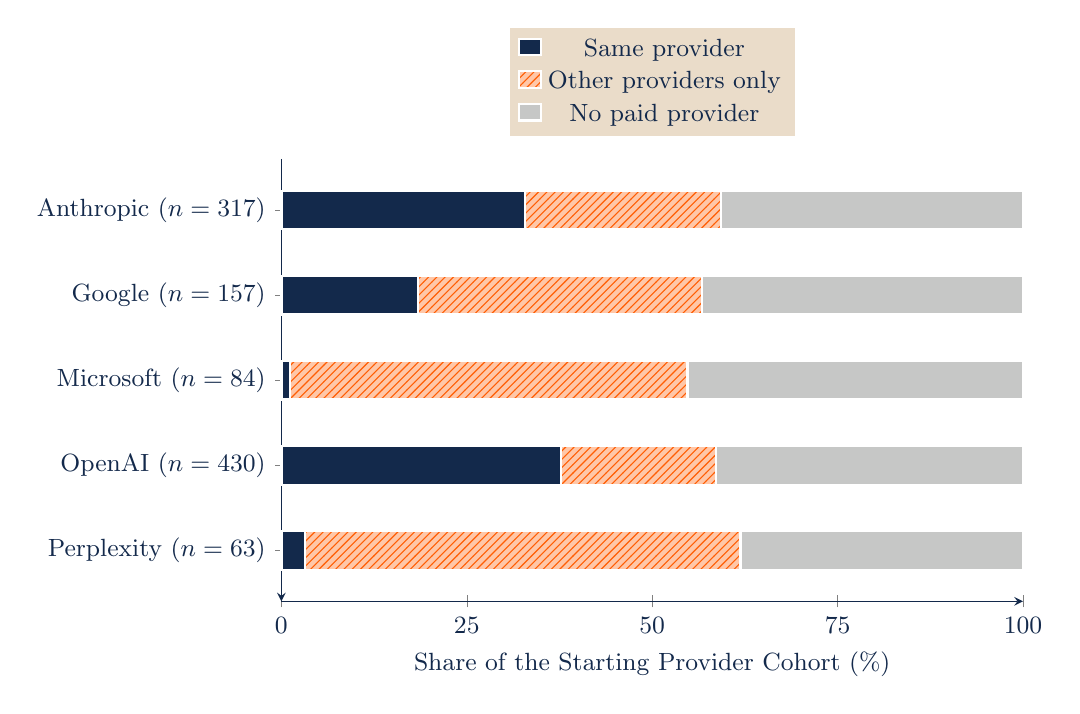
\begin{tikzpicture}
\begin{axis}[width=11cm,height=7.2cm,xbar stacked,bar width=14pt,
 xmin=0,xmax=100,ymin=-0.6,ymax=4.6,xtick={0,25,50,75,100},
 xlabel={Share of the Starting Provider Cohort (\%)},
 ytick={0,1,2,3,4},yticklabels={{Anthropic ($n=317$)},{Google ($n=157$)},{Microsoft ($n=84$)},{OpenAI ($n=430$)},{Perplexity ($n=63$)}},
 legend style={at={(0.5,1.05)},anchor=south,legend columns=1},
 y dir=reverse]
\addplot[fill=IlliniBlue,draw=white] coordinates {(32.807571,0.000000) (18.471338,1.000000) (1.190476,2.000000) (37.674419,3.000000) (3.174603,4.000000)};
\addplot[fill=IlliniOrange!35,draw=white,postaction={pattern=north east lines,pattern color=IlliniOrange}] coordinates {(26.498423,0.000000) (38.216561,1.000000) (53.571429,2.000000) (20.930233,3.000000) (58.730159,4.000000)};
\addplot[fill=LightStorm,draw=white] coordinates {(40.694006,0.000000) (43.312102,1.000000) (45.238095,2.000000) (41.395349,3.000000) (38.095238,4.000000)};
\legend{Same provider,Other providers only,No paid provider}
\end{axis}
\end{tikzpicture}

\end{adjustbox}
\endgroup
\par\medskip
{\small Entirely synthetic subscription panel. Provider labels identify simulated options.\par}
\note{These simulated percentages are not actual market shares or provider retention estimates. Multiple-provider behavior requires a definition that prevents incompatible categories from being added.

M4, Section 4.14, Marketing Analytics Lecture Notes. \url{../06_Lecture_Notes/modules/M04_Conjoint_Segmentation_and_CLV.md}}
\end{frame}
\begin{frame}{Subscriber Stocks and New Flows}
\usebeamercolor[fg]{normal text}
\vfill
\begin{slidebullets}
\item A subscriber stock includes past acquisition and survival.
\item A new-subscription flow can include first purchases and returns.
\item A price coefficient depends on the outcome and behavioral model.
\end{slidebullets}
\vfill
\note{Regressing subscriber stocks on current prices can combine persistent state with current choice. A structural interpretation must match the data-generating choice process.

M8, Section 8.13.2, Marketing Analytics Lecture Notes. \url{../06_Lecture_Notes/modules/M08_Current_Topics_and_Integrated_Decisions.md}}
\end{frame}
\begin{frame}{A Known Model Is a Useful Verification Case}
\usebeamercolor[fg]{normal text}
\centering
\begingroup
\begin{adjustbox}{max width=0.98\textwidth,max totalheight=0.65\textheight}
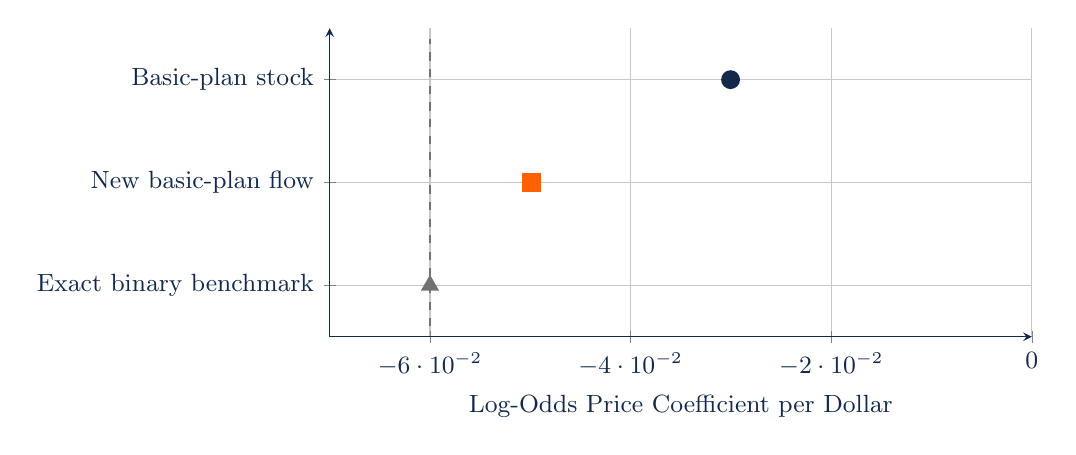
\begin{tikzpicture}
\begin{axis}[width=10.5cm,height=5.5cm,xmin=-0.07,xmax=0,ymin=-0.5,ymax=2.5,
 xlabel={Log-Odds Price Coefficient per Dollar},
 ytick={0,1,2},yticklabels={{Exact binary benchmark},{New basic-plan flow},{Basic-plan stock}},
 xtick={-0.06,-0.04,-0.02,0},scaled x ticks=false,grid=major]
\addplot[Storm,dashed] coordinates {(-0.06,-0.4) (-0.06,2.4)};
\addplot[IlliniBlue,mark=*,only marks,mark size=3pt] coordinates {(-0.03003875,2)};
\addplot[IlliniOrange,mark=square*,only marks,mark size=3pt] coordinates {(-0.04987365,1)};
\addplot[Storm,mark=triangle*,only marks,mark size=3pt] coordinates {(-0.06000000,0)};
\end{axis}
\end{tikzpicture}

\end{adjustbox}
\endgroup
\par\medskip
{\small Synthetic demand exercise with a known binary-model benchmark.\par}
\note{Recovering the benchmark checks implementation under its assumptions. It does not establish a structural interpretation for the richer simulated panel or actual market data.

M8, Section 8.13.1, Marketing Analytics Lecture Notes. \url{../06_Lecture_Notes/modules/M08_Current_Topics_and_Integrated_Decisions.md}}
\end{frame}
\begin{frame}{Seller Costs and Customer Alternatives}
\usebeamercolor[fg]{normal text}
\centering
\begingroup
\begin{adjustbox}{max width=0.98\textwidth,max totalheight=0.65\textheight}
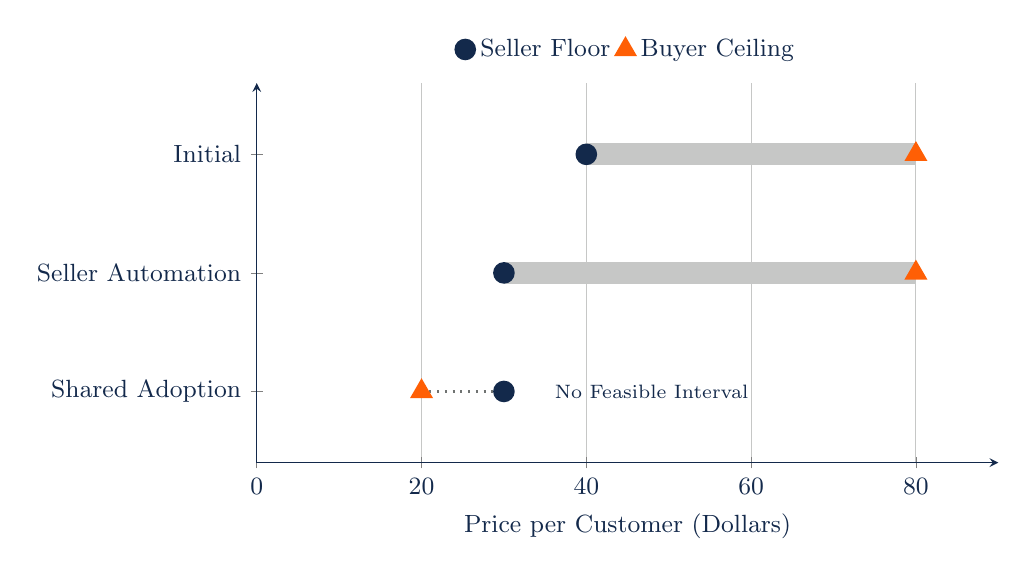
\begin{tikzpicture}
\begin{axis}[width=11cm,height=6.4cm,xmin=0,xmax=90,ymin=-.6,ymax=2.6,
xtick={0,20,40,60,80},ytick={0,1,2},
yticklabels={Shared Adoption,Seller Automation,Initial},
xlabel={Price per Customer (Dollars)},xmajorgrids=true,
legend style={at={(.5,1.03)},anchor=south,legend columns=2,fill=none}]
\addplot[LightStorm,line width=8pt,forget plot] coordinates {(40,2) (80,2)};
\addplot[LightStorm,line width=8pt,forget plot] coordinates {(30,1) (80,1)};
\addplot[Storm,dotted,forget plot] coordinates {(20,0) (30,0)};
\addplot[only marks,IlliniBlue,mark=*,mark size=3.5pt] coordinates {(40,2) (30,1) (30,0)};
\addlegendentry{Seller Floor}
\addplot[only marks,IlliniOrange,mark=triangle*,mark size=4pt] coordinates {(80,2) (80,1) (20,0)};
\addlegendentry{Buyer Ceiling}
\node[anchor=west,font=\scriptsize] at (axis cs:35,0) {No Feasible Interval};
\end{axis}
\end{tikzpicture}

\end{adjustbox}
\endgroup
\par\medskip
{\small Hypothetical dollars per customer, conditional on 50 sales.\par}
\note{Delivered value is 200 dollars, buyer burden 40, and fixed cost 1,000. Unit cost falls from 20 to 10. Outside-option utility then rises from 80 to 140. Gray intervals indicate simultaneous weak participation and cost recovery. Volume and valuations are imposed; these bounds neither estimate demand nor solve a pricing equilibrium. Customers are indifferent at the ceiling.

Marketing Analytics Lecture Notes, M8 §8.17.2.}
\end{frame}
\begin{frame}{AI Workflow Quality}
\usebeamercolor[fg]{normal text}
\vfill
\begin{slidebullets}
\item Measure the completed analysis and its validity.
\item Include generation, review, and repair time.
\item Use comparable tasks and independent quality criteria.
\end{slidebullets}
\vfill
\note{A time comparison can favor a tool because it abandons difficult tasks or reduces quality. The outcome definition should account for completion and validity before comparing speed.

M8, Section 8.6, Marketing Analytics Lecture Notes. \url{../06_Lecture_Notes/modules/M08_Current_Topics_and_Integrated_Decisions.md}}
\end{frame}
\begin{frame}{Review Time Is Part of Production}
\usebeamercolor[fg]{normal text}
\centering
\begingroup
\fontsize{11}{13.2}\selectfont
\def\small{\fontsize{10}{12}\selectfont}
\def\footnotesize{\fontsize{9}{11}\selectfont}
\def\scriptsize{\fontsize{8}{9.5}\selectfont}
\hyphenpenalty=10000
\begin{adjustbox}{max width=0.98\textwidth,max totalheight=0.65\textheight}
% Original synthetic teaching figure; see corresponding module.
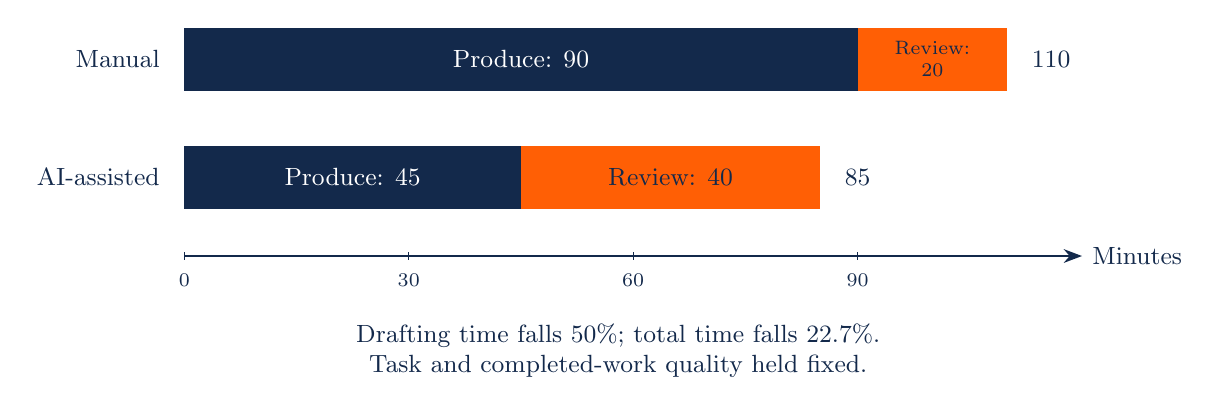
\begin{tikzpicture}[x=.095cm,y=1cm]
\node[anchor=east] at (-2,1.5) {Manual};\node[anchor=east] at (-2,0) {AI-assisted};
\fill[IlliniBlue] (0,1.1) rectangle (90,1.9);\fill[IlliniOrange] (90,1.1) rectangle (110,1.9);
\fill[IlliniBlue] (0,-.4) rectangle (45,.4);\fill[IlliniOrange] (45,-.4) rectangle (85,.4);
\node[text=white] at (45,1.5) {Produce: 90};\node[text=IlliniBlue,font=\scriptsize,align=center] at (100,1.5) {Review:\\20};
\node[text=white] at (22.5,0) {Produce: 45};\node[text=IlliniBlue] at (65,0) {Review: 40};
\node[anchor=west] at (112,1.5) {110};\node[anchor=west] at (87,0) {85};
\draw[edge] (0,-1)--(120,-1) node[right] {Minutes};
\foreach \x in {0,30,60,90} {\draw[IlliniBlue] (\x,-1.05)--(\x,-.95);\node[anchor=north,font=\scriptsize] at (\x,-1.1) {\x};}
\node[align=center,text width=12cm] at (58,-2.2) {Drafting time falls 50\%; total time falls 22.7\%.\\Task and completed-work quality held fixed.};
\end{tikzpicture}

\end{adjustbox}
\endgroup
\par\medskip
{\small Synthetic workflows meet the same stated quality requirement.\par}
\note{The manual workflow uses 90 minutes to produce and 20 to review. The assisted workflow uses 45 and 40. These are imposed time inputs, not an estimate of a universal AI effect.

M8, Section 8.6, Marketing Analytics Lecture Notes. \url{../06_Lecture_Notes/modules/M08_Current_Topics_and_Integrated_Decisions.md}}
\end{frame}
\begin{frame}{Reuse Has a Break-Even Workload}
\usebeamercolor[fg]{normal text}
\centering
\begingroup
\begin{adjustbox}{max width=0.98\textwidth,max totalheight=0.65\textheight}
\begin{tikzpicture}
\begin{axis}[width=12cm,height=6.4cm,xmin=0,xmax=25,ymin=0,ymax=52,
xtick={0,6,12,18,24},ytick={0,12,24,36,48},xlabel={Comparable Uses in the Quarter},
ylabel={Total Work (Hours)},ymajorgrids=true,
legend style={at={(.5,1.03)},anchor=south,legend columns=2,fill=none}]
\addplot[IlliniBlue,mark=*,mark repeat=6,mark size=2.5pt] table[col sep=comma,x=uses,y=old_hours]
{../03_Data_and_Code/AI_Workflows/results/reuse_costs.csv};
\addlegendentry{Existing Process}
\addplot[IlliniOrange,dashed,mark=square*,mark repeat=6,mark size=2.5pt] table[col sep=comma,x=uses,y=reusable_hours]
{../03_Data_and_Code/AI_Workflows/results/reuse_costs.csv};
\addlegendentry{Reuse, Setup, and Upkeep}
\draw[Storm,dotted] (axis cs:12,0)--(axis cs:12,24);
\node[anchor=north west,font=\scriptsize] at (axis cs:12.4,22) {Break-Even: 12 Uses};
\end{axis}
\end{tikzpicture}

\end{adjustbox}
\endgroup
\par\medskip
{\small Hypothetical equal-quality work: six setup hours, with adaptation included.\par}
\note{Execution alone falls from two hours to 1.25, but 0.25 upkeep hours are required per use. Net savings become positive at the thirteenth use. Twenty-four uses save six hours, a 12.5\% reduction after setup and upkeep. The numbers are imposed and do not measure course development time. Run investment.py and vary upkeep or workload.

Marketing Analytics Lecture Notes, M8 §8.17.1.}
\end{frame}
\begin{frame}{Model Updates and Unresolved Tasks}
\usebeamercolor[fg]{normal text}
\vfill
\begin{slidebullets}
\item Connect an update to a recorded difficulty and a feasible comparison.
\item Evaluate the frozen challenger and current procedure on fresh cases.
\item Include setup, correction, and maintenance in the adoption decision.
\end{slidebullets}
\vfill
\note{Record actual access, supported inputs, failure conditions, and the original decision. A difficulty register can omit an unexpected useful route, so allow exploratory comparisons and revise the diagnosis. Retain the existing procedure when the challenger provides no supported improvement. A new schema or customer population can require revalidation of a retained helper.

Marketing Analytics Lecture Notes, M8 §8.18.}
\end{frame}
\begin{frame}{A Choice Procedure Can Change Renewal}
\usebeamercolor[fg]{normal text}
\vfill
\begin{slidebullets}
\item A direct offer and an offer preceded by questions can produce different choices.
\item The customer still makes the final selection.
\item An independent value measure determines whether an additional renewal benefits that customer.
\end{slidebullets}
\vfill
\note{Questions, defaults, or retention prompts can precede a fixed target decision. The welfare comparison depends on consumer values, stable response probabilities, and the procedure set. A renewal increase alone does not establish either benefit or harm.

M8, Section 8.14, Marketing Analytics Lecture Notes. \url{../06_Lecture_Notes/modules/M08_Current_Topics_and_Integrated_Decisions.md}}
\end{frame}
\begin{frame}{Opposed Interests}
\usebeamercolor[fg]{normal text}
\noindent Suppose renewal yields firm margin $\nu>0$ and costs the customer $\sigma>0$ relative to declining.
\medskip
\[
\Delta\Pi=\nu(s-s_0),\qquad \Delta V=-\sigma(s-s_0)
\]
\medskip
\noindent A higher renewal probability raises profit and lowers customer value under these stated stakes.
\note{This conditional comparison holds the offer, monetary values, and relevant response population fixed. It does not infer customer harm from conversion alone. Additional time and authority costs require separate measurement.

M8, Section 8.14, Marketing Analytics Lecture Notes. \url{../06_Lecture_Notes/modules/M08_Current_Topics_and_Integrated_Decisions.md}}
\end{frame}
\begin{frame}{Profit and Customer Value Can Move Oppositely}
\usebeamercolor[fg]{normal text}
\centering
\begingroup
\begin{adjustbox}{max width=0.98\textwidth,max totalheight=0.65\textheight}
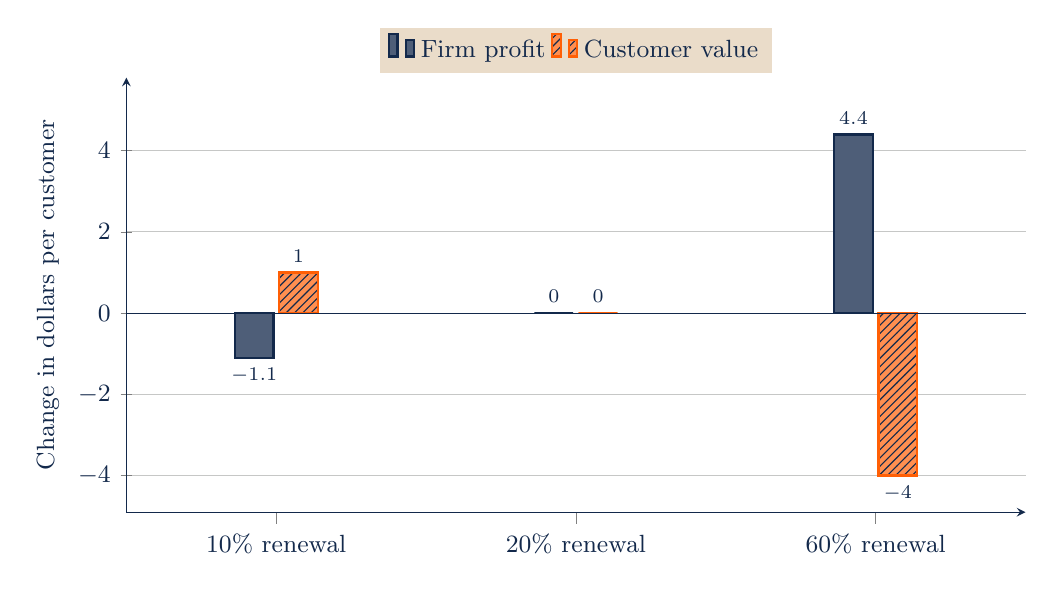
\begin{tikzpicture}
\begin{axis}[
  width=13cm,height=7.1cm,
  ybar,bar width=14pt,
  ymin=-4.9,ymax=5.8,
  ylabel={Change in dollars per customer},
  symbolic x coords={Low,Direct,High},
  xtick=data,xticklabels={10\% renewal,20\% renewal,60\% renewal},
  enlarge x limits=0.25,
  ytick={-4,-2,0,2,4},ymajorgrids=true,
  legend style={at={(0.5,1.01)},anchor=south,legend columns=2},
  nodes near coords,nodes near coords style={font=\scriptsize},
  axis x line*=bottom,axis y line*=left]
\addplot[draw=IlliniBlue,fill=IlliniBlue!75] coordinates {(Low,-1.1) (Direct,0) (High,4.4)};
\addplot[draw=IlliniOrange,fill=IlliniOrange!70,postaction={pattern=north east lines,pattern color=IlliniBlue}] coordinates {(Low,1) (Direct,0) (High,-4)};
\legend{Firm profit,Customer value}
\draw[IlliniBlue,thin] (rel axis cs:0,0.45794)--(rel axis cs:1,0.45794);
\end{axis}
\end{tikzpicture}

\end{adjustbox}
\endgroup
\par\medskip
{\small Synthetic probabilities and fixed stakes. Direct renewal is 20\%.\par}
\note{The direct-choice benchmark is distinct from the consumer-preferred procedure. Relative to the 10\% procedure, the 60\% procedure creates a 5-dollar customer loss. These probabilities and monetary values are imposed inputs, not observed customer responses.

M8, Section 8.14, Marketing Analytics Lecture Notes. \url{../06_Lecture_Notes/modules/M08_Current_Topics_and_Integrated_Decisions.md}}
\end{frame}
\begin{frame}{Experimentation Selects the Commercial Winner}
\usebeamercolor[fg]{normal text}
\vfill
\begin{slidebullets}
\item A fixed set of procedures has stable renewal probabilities.
\item Independent randomized samples estimate each probability.
\item With opposed interests, accurately selecting the largest rate also selects the largest loss in that set.
\end{slidebullets}
\vfill
\note{The result requires common fixed stakes, a fixed catalog chosen before the experiment, stable responses from experiment to deployment, and complete independently sampled outcomes. It does not say that every experiment harms consumers.

M8, Section 8.14, Marketing Analytics Lecture Notes. \url{../06_Lecture_Notes/modules/M08_Current_Topics_and_Integrated_Decisions.md}}
\end{frame}
\begin{frame}{A Cancellation Evaluation}
\usebeamercolor[fg]{normal text}
\vfill
\begin{slidebullets}
\item Include a direct-cancellation comparison.
\item Record whether optional retention content can be refused before exposure.
\item Measure completion, elapsed time, subsequent charges, and customer value.
\end{slidebullets}
\vfill
\note{An effective refusal path and an independent value measure reveal dimensions hidden by renewals. A direct-choice arm helps isolate the effect of the preceding interaction.

M8, Section 8.14, Marketing Analytics Lecture Notes. \url{../06_Lecture_Notes/modules/M08_Current_Topics_and_Integrated_Decisions.md}}
\end{frame}
\begin{frame}{Retention Leaves the Mechanism Unresolved}
\usebeamercolor[fg]{normal text}
\centering
\begingroup
\fontsize{11}{13.2}\selectfont
\def\small{\fontsize{10}{12}\selectfont}
\def\footnotesize{\fontsize{9}{11}\selectfont}
\def\scriptsize{\fontsize{8}{9.5}\selectfont}
\hyphenpenalty=10000
\begin{adjustbox}{max width=0.98\textwidth,max totalheight=0.65\textheight}
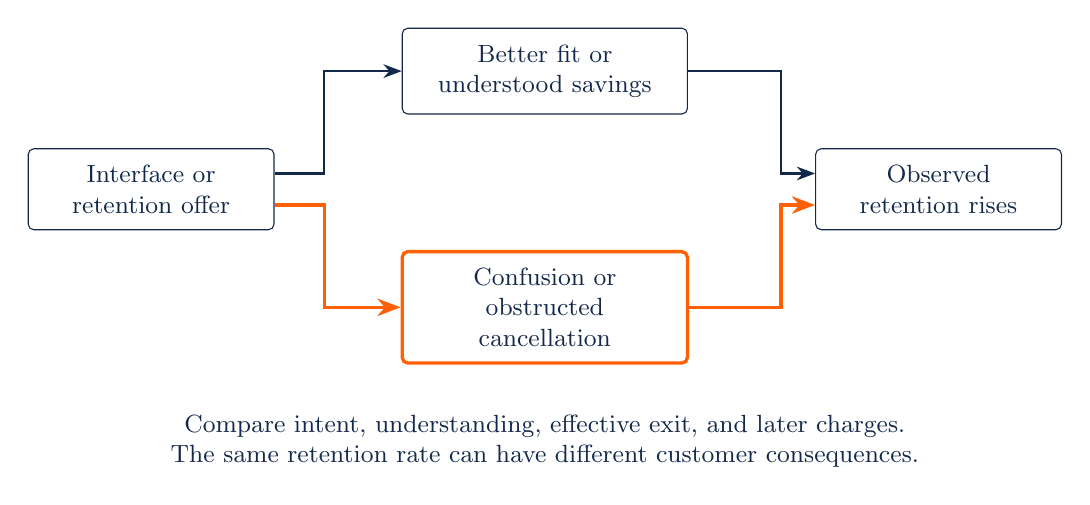
\begin{tikzpicture}
\node[box,text width=2.7cm] (design) at (0,0) {Interface or\\retention offer};
\node[box,text width=3.2cm] (value) at (5,1.5) {Better fit or\\understood savings};
\node[orangebox,text width=3.2cm] (friction) at (5,-1.5) {Confusion or\\obstructed cancellation};
\node[box,text width=2.7cm] (retention) at (10,0) {Observed\\retention rises};
\draw[edge] ([yshift=.2cm]design.east)--(2.2,.2)--(2.2,1.5)--(value.west);
\draw[accent] ([yshift=-.2cm]design.east)--(2.2,-.2)--(2.2,-1.5)--(friction.west);
\draw[edge] (value.east)--(8,1.5)--(8,.2)--([yshift=.2cm]retention.west);
\draw[accent] (friction.east)--(8,-1.5)--(8,-.2)--([yshift=-.2cm]retention.west);
\node[align=center,font=\small] at (5,-3.2) {Compare intent, understanding, effective exit, and later charges.\\The same retention rate can have different customer consequences.};
\end{tikzpicture}

\end{adjustbox}
\endgroup
\par\medskip
{\small The same payment outcome can follow valuable service or obstructed exit.\par}
\note{This is a conceptual diagram, not an estimated causal graph. It motivates collecting customer-outcome measures alongside retention. Existing M8 Section 8.14 supplies a fully specified synthetic welfare calculation; Section 8.19 connects the mechanism to recent policy and research.

\url{../01_Resources/13_Consumer_Agency_and_Recent_Research/Policy/README.md}}
\end{frame}
\begin{frame}{Federal Cancellation Policy: Current Status}
\usebeamercolor[fg]{normal text}
\vfill
\begin{slidebullets}
\item July 2025: the Eighth Circuit vacated the 2024 FTC rule.
\item February 2026: the FTC restored the earlier prenotification rule.
\item March 2026: an advance notice sought input on possible amendments.
\end{slidebullets}
\vfill
\note{Checked November 5, 2026. The court identified a procedural deficiency. The March notice does not establish a replacement obligation; the October 14 information-collection notice concerns the restored rule. ROSCA separately requires disclosure, express informed consent, and simple cancellation mechanisms for covered online negative-option transactions.

\url{../01_Resources/13_Consumer_Agency_and_Recent_Research/Policy/README.md}}
\end{frame}
\begin{frame}{Cancellation Rules Differ by Jurisdiction}
\usebeamercolor[fg]{normal text}
\vfill
\begin{slidebullets}
\item California strengthened its Automatic Renewal Law on July 1, 2025.
\item New York City's separate rule took effect October 1, 2026.
\item Identify covered transactions, enrollment media, and sector exceptions.
\end{slidebullets}
\vfill
\note{California guidance describes online cancellation without obstruction for online enrollment. NYC Section 5-110.2 requires simple cancellation as easy as enrollment and bars obstruction or unreasonable delay. Retention offers are subject to those restrictions; Section 5-110.3 contains sector exclusions. These sources were checked November 5, 2026. See M8 Section 8.19.

\url{../01_Resources/13_Consumer_Agency_and_Recent_Research/Policy/README.md}}
\end{frame}
\begin{frame}{Research Frequency and Policy Importance}
\usebeamercolor[fg]{normal text}
\vfill
\begin{slidebullets}
\item Social influence leads the selected literature clusters.
\item Exit friction can affect many customers even with few papers in the sample.
\item Choose safeguards using mechanism, exposure, and customer consequences.
\end{slidebullets}
\vfill
\note{Journal counts give each paper equal weight and do not measure market exposure or loss. The 48-paper primary sample is access-selected and largely coded for inferred dual use. The full DOI census contains 824 eligible records with 721 full-text gaps. See M4 Section 4.17 and M8 Section 8.19.

\url{../03_Data_and_Code/Consumer_Agency_Literature/README.md}}
\end{frame}
\begin{frame}{Pricing, Reviews, and Delivery}
\usebeamercolor[fg]{normal text}
\vfill
\begin{slidebullets}
\item Price-display rules require attention to the covered industry.
\item Reviews presented as customer experiences require truthful provenance.
\item Housing-ad delivery can create discrimination concerns beyond targeting choices.
\end{slidebullets}
\vfill
\note{The FTC fee rule covers live-event tickets and short-term lodging. Its review rule distinguishes business creation and purchase of false reviews from mere hosting. The DOJ Meta settlement addresses housing advertising specifically. These sources do not establish an identical rule for every marketing application.

Primary-source scope and status record: \url{../06_Lecture_Notes/ETHICS_AND_REGULATION.md.}}
\end{frame}
\begin{frame}{Pricing Language and Regulatory Evidence}
\usebeamercolor[fg]{normal text}
\vfill
\begin{slidebullets}
\item Shelf infrastructure, price rules, and consumer effects are separate objects.
\item The FTC's January 2025 report describes research on pricing intermediaries.
\item Specify the practice and applicable authority before making a legal claim.
\end{slidebullets}
\vfill
\note{The US FTC Section 6(b) staff research summaries report preliminary findings. This research publication has no rule effective date and supplies no legal finding against firms in the earnings-call sample. Use the source-linked cases from M5 to identify operational facts still needed.

M8, Section 8.16. FTC, January 2025, pp. 1–3. \url{https://www.ftc.gov/system/files/ftc_gov/pdf/p246202_surveillancepricing6bstudy_researchsummaries_redacted.pdf}}
\end{frame}
\begin{frame}[fragile]{A Welfare Comparison}
\usebeamercolor[fg]{normal text}
\noindent Synthetic stakes distinguish profit from customer value.
\begin{lstlisting}
direct, selected = 0.20, 0.60
firm_margin, customer_loss = 11, 10
firm_gain = firm_margin * (selected-direct)
value_change = -customer_loss * (selected-direct)
assert round(firm_gain, 2) == 4.40
assert round(value_change, 2) == -4.00
\end{lstlisting}
{\small Higher combined surplus can coexist with a customer loss under these assumptions.\par}
\note{The combined change is 0.40 dollars per potential customer in this example. The welfare result is conditional on the imposed values. A choice probability does not independently reveal those values.

M8, Section 8.14, Marketing Analytics Lecture Notes. \url{../06_Lecture_Notes/modules/M08_Current_Topics_and_Integrated_Decisions.md}}
\end{frame}
\begin{frame}{Coding Exercise: A Marketing Evaluation}
\usebeamercolor[fg]{normal text}
\vfill
\begin{slidebullets}
\item Calculate reuse break-even and the conditional price interval.
\item Compute profit and customer value for alternative retention procedures.
\item Propose an interface change and the evidence needed to evaluate it.
\end{slidebullets}
\vfill
\note{Run ../03\_Data\_and\_Code/Lecture\_Examples/session\_examples.py S14 and S14\_ethics. The GenAI demand programs provide richer stock, flow, cohort, and benchmark checks. Keep empirical measurements separate from imposed welfare inputs. The AI\_Workflows folder supplies complete standard-library calculations with synthetic inputs.

M8, Section 8.13.3, Marketing Analytics Lecture Notes. \url{../06_Lecture_Notes/modules/M08_Current_Topics_and_Integrated_Decisions.md}}
\end{frame}
\begin{frame}{A Decision With Consumer Outcomes}
\usebeamercolor[fg]{normal text}
\vfill
\begin{slidebullets}
\item State the commercial target and customer outcome.
\item Identify the procedure the customer can accept, refuse, or revise.
\item Connect the proposed action to current rules and supporting evidence.
\end{slidebullets}
\vfill
\note{A marketing policy can improve matching, convenience, and customer value. Its evaluation should also reveal when additional sales come from misleading claims, unwanted friction, or conflicting incentives.

Primary-source scope and status record: \url{../06_Lecture_Notes/ETHICS_AND_REGULATION.md.}}
\end{frame}
\end{document}
